%*****************************************************************************************
%*********************************** First Chapter ***************************************
%*****************************************************************************************

\chapter{Motivation}  %Title of the First Chapter

\epstopdfsetup{outdir=Chapter1/Figs/PDF/}
\ifpdf
    \graphicspath{{Chapter1/Figs/Raster/}{Chapter1/Figs/PDF/}{Chapter1/Figs/}}
\else
    \graphicspath{{Chapter1/Figs/Vector/}{Chapter1/Figs/}}
\fi

The purpose of this project is to create a chromatic skin and feature detector for application in mobile devices. Using a given device's built-in CCD camera, objects with characteristics matching those of human skin are identified. This presents a number of challenges. Since we are trying to use the chromatic information of human skin to distinguish objects (e.g. hands, fingers) in a given scene, working in a chromatic space helps to simplify this problem. A chromatic space is a color space wherein the color information is laid out in as few dimensions as possible, with a separate dimension for luminosity --- the brightness information. Fundamentally, the issue with this is that CCD cameras capture information using RGB values which mixes the chromatic information with the luminosity. Separating this information is the first part of the challenge.

The second part of the challenge is, because we are searching for objects which exhibit certain chromatic characteristics, a statistical model must be developed and applied in order to characterize the objects as such.

The third and final challenge is developing efficient, discrete maths to perform the chromatic space rotation and to apply the statistical model efficiently enough such that all the chromatic information about the target object is retained, whilst all irrelevant information is discarded.

While several people have developed algorithms for skin detection, their focus has been squarely on detection rather than retention of information. For color spaces, Hue- based spaces, such as HSV, have been used due to the clear separation of the chromatic information and luminosity <Zarit and Sigal>. Simpler color spaces, such as Normalized RGB, have been used in video applications due to the demand of continuously processing image frames <Soriano>. As for gathering statistics, histogram thresholding <Soriano and Sigal> and Gaussian models using 2D Gaussians <Terrillon>, 3D Gaussians or multiple Gaussian clusters <Veshnevets> are among the most common models in practice <Shin>, though other models have been used to similar effect, such as the Self-Organizing Map (SOM) in <Brown>'s application. Additionally, practically every application uses double precision numbers in their transformations <Shin, Veshnevets and Terrillon>.

Regardless of the color spaces and statistical models used, all of these algorithms have the same fundamental approach: the image is transformed into some color space, and the statistical model is applied, resulting in a binary image which classifies whether any given pixel is skin. This information is then used as a mask and applied to the original image. This algorithm is fundamentally different to the one used for this project; the primary goal is to preserve information about the skin, as opposed to simply detecting whether a given object is skin or not. We process the image into a new chromatic space, then apply the statistical model, resulting in an image which contains all the chromatic and luminosity information about the skin within it, and information about non-skin areas is lost. 

We are preserving the information in a targeted way, reducing the overall information in the image whilst preserving the relevant information about the object we're interested in. This is a clear difference from the more common binary categorization approach, though it is possible to adapt our approach to the same process. However, as it stands, the entire process is more efficient than the first step in a binary classifier, and should be faster than moving to an HSV (Hue, Saturation and Value) image using standard library routines.


\section{Choosing a Color Space}

As mentioned previously, one of the challenges facing this project is identifying a chromatic space in which the color information and luminosity from the raw RGB image can be separated, thereby simplifying the process of identification of human skin color. To this end, the most widely-used chromatic spaces in practical applications of skin color classification have been evaluated --- HSV, LAB and YCbCr --- all of which have a number of readily-available implementations (\cite{Vezhnevets2003,Zarit1999a,Yang1997a,Brand2000a,Sigal2000a,Chai2000a,Phung2002a}).

Unlike RGB, the HSV color space makes a clear distinction between the chrominance (the "Hue" and "Saturation" channels) and the luminance (the "Value" channel), storing them separately (\cite{Vezhnevets2003,Sigal2000a}). However, the chromatic information in the Hue channel is expressed in polar coordinates, thereby necessitating a coordinate transform when converting from the raw image data. Given the nature of the algorithm outlined herein --- targeted preservation of information, as opposed to classification ---  the computational cost of this transformation is undesirable.

LAB and YCbCr, on the other hand, explicitly separate the chrominance and luminance without an accompanying polar coordinate transform (\cite{Vezhnevets2003,Poynton1997,Phung2002a}). LAB and YCbCr use a matrix transform to convert from RGB, allowing for simple and quick conversion exploiting optimised matrix multiplication routines. However, while they appear to be perfectly suited for the purposes of this project, a number of issues arise when represented discretely. LAB, YCbCr and other such luminosity-chrominance spaces all include implicit white-point correction in the readily-available implementations, which distorts the information from the raw image. Also, while the transform is reversible mathematically, discrete data types are used in practical computer science applications, and in most implementations the output is the same data type as the input, resulting in some loss of information when the transform is applied.

Furthermore, based on the skin statistics we have gathered --- which will be described in detail in the next chapter --- the entire region of skin color in the chromatic space can be expressed as a 2D Gaussian. Typically, this is a complex operation, but by aligning the chromatic axes of a luminosity-chrominance space with the major and minor axes of the 2D Gaussian, it can be expressed as the product of two 1D Gaussians in each chromatic channel, thereby facilitating the application of the statistics. It was decided that a bespoke color space would be best suited for this project. 

This new bespoke color space transformation will fulfil the following design criteria:

\begin{itemize}
\item Be expressible as a matrix transformation of the RGB values.
\item Allow an arbitrary orientation of the chromatic axis.
\item Be expressed as an integer type at every step of the transformation, eliminating floating point operations and allowing for efficient optimization on mobile processors.
\item Allow for retention and elimination of color space information, to be performed in a non-linear fashion using a statistical specification of the redistribution based on a normal distribution.
\end{itemize}


\section{Physiology Study}\label{sec:PhysiologyStudy}

\subsection{Chromophores in the Skin}

Now that we have chosen our chromatic space, we will look at the necessary biological considerations. Specifically, the chromophores in human skin and how they affect how skin appears to different detection devices. In brief, chromophores are chemicals in the skin which act as an optical barrier to light by means of scattering and absorption <Anderson, Parrish>. In the case of human skin, the chemicals responsible for both are different; the absorption chemicals affect the color, while the scattering chemicals determine the average path length of the light through the skin, thereby determining the amount of light which is absorbed. The longer the path length, the more light is absorbed for any given concentration of a chromophore. 

While there are a variety of chromophores, we will be focusing on the four which most significantly effect skin color: oxy-hemoglobin, deoxy-hemoglobin, eumelanin and pheomelanin. The absorption spectra for these chromophores are known quantities, which we can use to find the absorbance of skin, "absorbance" in this case being the ratio of reflected light to absorbed light. The absorbance can be found by applying Beer-Lambert Law <web page ref here>:

\begin{equation}\label{eq:BeerLambert}
A = \log \frac{I_{0}}{I} = \epsilon l  c 
\end{equation}

Where $A$ is the absorbance, $I_{0}$ is the intensity of the light passing through the reference cell, $I$ is the intensity of the light passing through the sample cell, $l$ is the path length of light through the skin, and $c$ is the concentration of the chromophore. $\epsilon$ is variously called "molar absorptivity," the "molar extinction coefficient," and the "molar absorption coefficient;" all equivalent terms for how strongly a chemical species absorbs light at a given wavelength.

In order to apply the molar absorptivity, we need the average path length of skin, the average concentration of the chromophore, and their Beer-Lambert Law relation --- in this case, the product of them all. Unfortunately, the units are not consistent <web page ref here>, but they can each be converted into the SI units, $m^{2}/mo$. The data on the chromophores were obtained from the OMLC website, which contains information on the absorption spectra for many different chemicals, including the aforementioned four skin chromophores. 

So, our first task is to convert everything into consistent SI units, and then find the absorbance of the skin using the Beer-Lambert Law relation.

\subsection{Response Spectra}

The response spectrum is how a given sensor --- such as the human eye or a CCD --- responds to very specific wavelengths of light. Essentially, it is the raw output from the sensor. This is almost never used, and is generally inaccessible even at the hardware layer, as the circuitry very close to the CCD does a basic level of color rebalancing. As we don't know the full color correction for every possible CCD, we observed the raw output spectra of several different devices and then tried two very simple methods of rebalancing the color:

The first is peak normalization, which simply levels out the maximum output in each channel such that the peak output for each of the channels is equal. This approach is very simple, but is quite likely from an electrical engineering perspective as it facilitates the digitization of the color information.

The second method is to approach the response spectra as the basis functions for representing the spectrum. Using this approach, each basis function is normalized according to its integral over the visible wavelengths, giving an equal weighting to each of the response spectra functions over the range of values, rather than focusing on a peak value. Mathematically speaking, this approach is not unusual when constructing a basis set as it facilitates the maths.


\begin{figure}[h!]
  \centering
    
\includegraphics[width=0.99\textwidth]{Chapter1/Figs/ResponseSpectrum_NokiaN900.eps}
    \caption{The response spectrum for the Nokia N900. }  \label{fig:ResponseSpectumNokia}
\end{figure}



It should be noted that the color balancing methods used in modern CCD devices are much more sophisticated than either of these approaches.

However, because the methods chosen here are straightforward amplifications of each channel, they're likely to be used as a first step in color rebalancing at the hardware level in the device. While we are not concerned with device constructions, it is useful to know how these devices capture the color information if this algorithm is to be used diagnostically, as color rebalancing may introduce artefacts and distortions in the data.


\begin{figure}[h!]
  \centering
    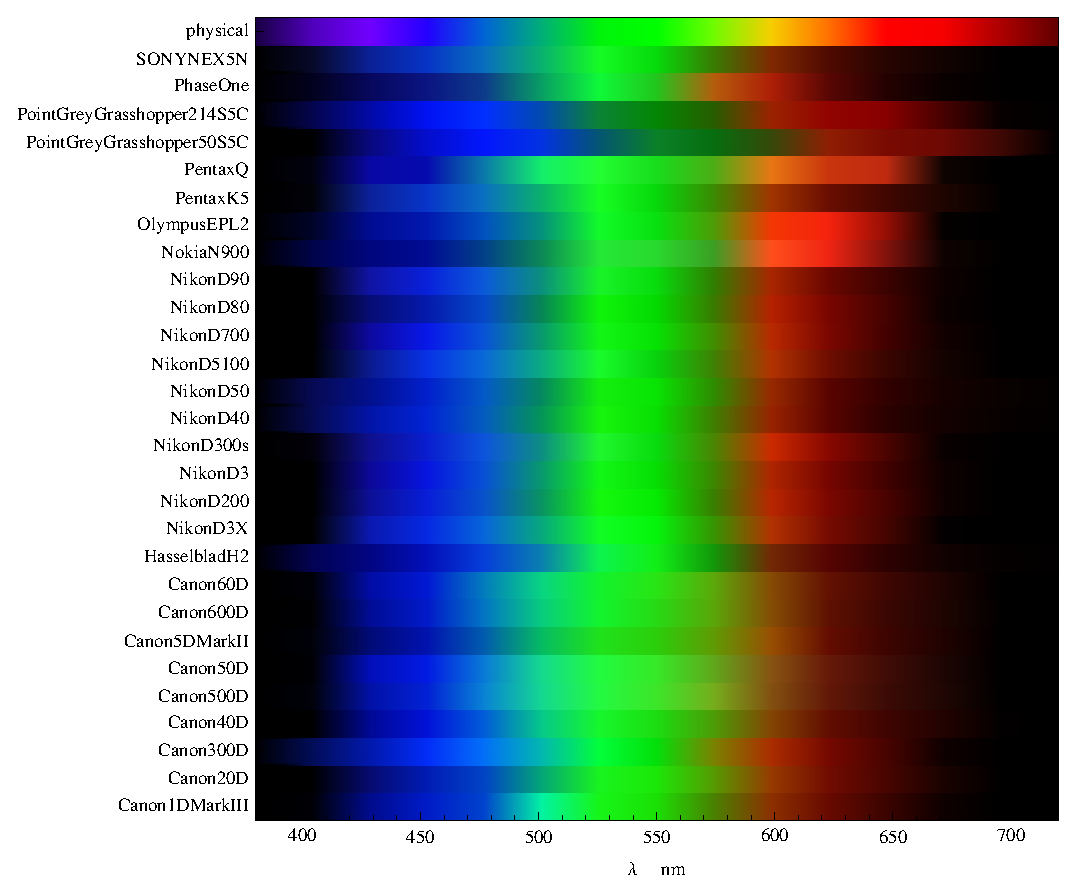
\includegraphics[width=0.99\textwidth]{Chapter1/Figs/ResponseSpectraStripes.eps}
    \caption{The light spectrum as viewed using various CCDs with a physical spectrum for comparison }  \label{fig:ResponseSpectraStripes}
\end{figure}

\begin{figure}[h!]
  \centering
    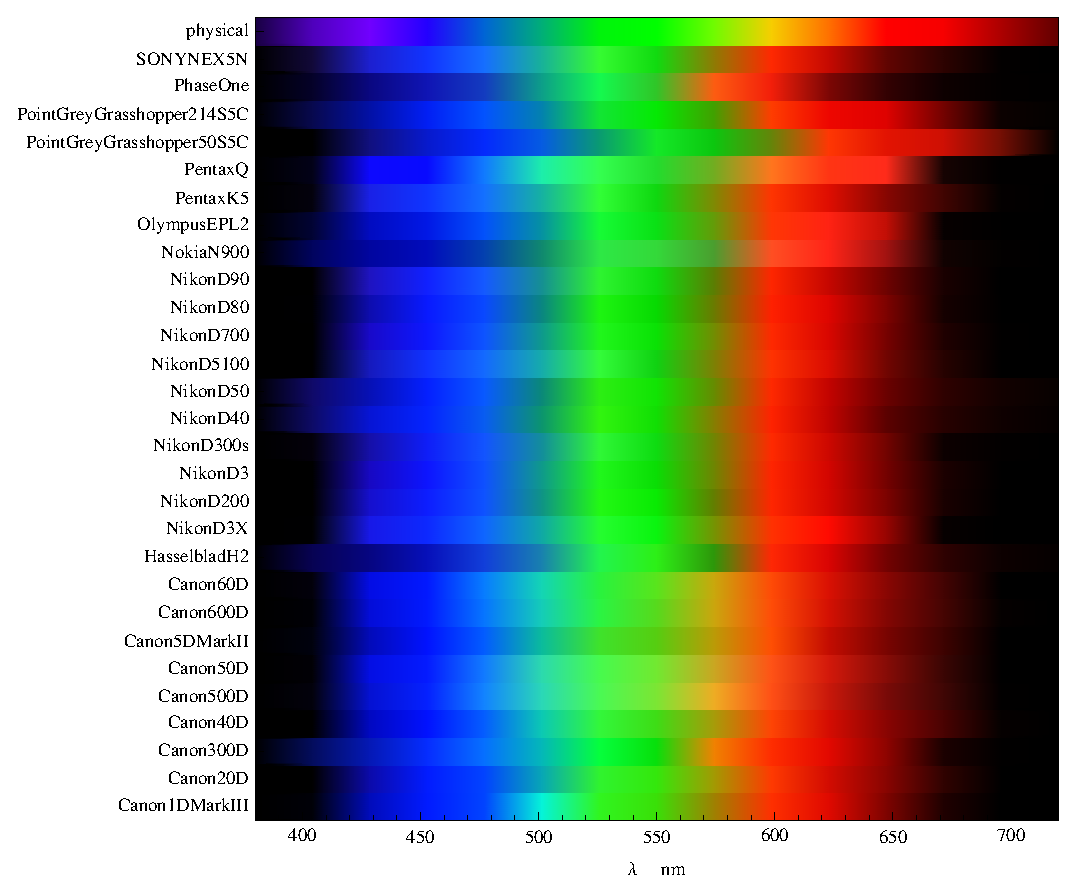
\includegraphics[width=0.99\textwidth]{Chapter1/Figs/ResponseSpectraStripesNorm.eps}
    \caption{The light spectrum as viewed using various CCDs after normalisation with a physical spectrum for comparison.}  \label{fig:ResponseSpectraStripesNorm}
\end{figure}
<graphical representation of the raw data of some CCDs from the site, illustrating where the information is captured>

Although we consider these sensors to be capturing information throughout the entire visible spectrum, what they are actually capturing varies quite significantly between devices. However, as these devices use the aforementioned color rebalancing algorithms to alter the image to look more sensible to human eyes, these differences aren't so apparent to us.

In addition to the color rebalancing, which corrects the behavior of the CCD devices, as is found in later sections <reference chapter 2>, some devices, like the iPhone, also apply a dynamic color rebalancing which attempts to even out the colors based on the image captured. This feature is intended to correct for strange lighting conditions and other such problems which could affect the image. This will be addressed in detail in <Chapter 2 reference again>.


\subsection{Skin Color Simulation}

So, we have the morlar absorptivity for the four key chromophores in the skin, we have the response spectra for a variety of devices, and a response spectra which serves as a target color output for all the devices after the color correction has been applied. Additionally, we are using the CIE 1931 RGB color space for the absorption spectra, which is closer to how our eyes perceive color than any other color space <reference here, mentioning the site with the spectrum data>. This means that, in principle, we can get appropriate RGB values for the four key chromophores at the hardware layer using the device response spectra, or at the AP layer using the CIE 1931 RGB color space spectrum <reference for CIE 1931 page here>, assuming the device's color space correction does its job. The question now is how to actually simulate skin color.

We can convert the molar absorptivity into an absorption spectrum for a chromophore if we know the average path length in the skin. So, the scattering properties of the skin will determine the path length. Since we are not trying to simulate any skin in particular, we can simply use average values taken from the <Camera Spectral Sensitivity Database project reference here>. At this point, we aren't so much interested in the saturation --- the concentration and path length both affect the saturation of the color rather than the hue --- as we are interested in the relative position around the luminosity axis; we want the saturation to lie on the axis.

So now we have an absorption spectrum, but the color that we perceive is the light which is re-emitted, and that is what we are really interested in: the re-emitted light, or $R$. While the optics is a complicated study, there is a relatively simple theory called Kubelka-Munk Theory, which allows us to turn an absorption spectra into a re-emission spectra:

\begin{equation}\label{eq:KubelkaMunk}
r=\frac{A}{S}
r=\frac{(R-1)^2-T^2}{2 R}
S=\frac{\tanh ^{-1}\left(\frac{\sqrt{r (r+2)} R}{1-(r+1) R}\right)}{d \sqrt{r (r+2)}}
\end{equation}

Where $A$ is the absorption, $S$ is the scattering of light, $R$ is the re-emission, and $T$ is transmittance. As the transmittance $T$ of human skin is approximately zero at visible wavelengths, $\frac{A}{S}$ can be expressed as:

\begin{equation}\label{eq:KubelkaMunk2}
\frac{A}{S}=\frac{(R-1)^2}{2 R}
\left\{\left\{R\to -\sqrt{r^2+2 r}+r+1\right\},\left\{R\to \sqrt{r^2+2 r}+r+1\right\}\right\}
\end{equation}

As $r$ is $\frac{A}{S}$, the re-emission $R$ must go down with increasing absorption $A$:

<figure showing graph here>

As for finding the RGB values, the bright color is the response of the CCD. By integrating the following functions in the figure below, we get the channel output:

<Figures along with notes on the brown translucent function showing the light coming in (the chromophore), the light colored one (response function)>

Thus, we can now find the channel output for any device we have a response function for.

At this point, we're going from the physical space to a virtual space; we have a physical quantity, the energy of light, and we are turning it into three numbers. The output depends on the measuring device. In the case of the human eye, it has a certain response based on the chemistry of the cones, and our retina produces the signal. However, there are only three different types of cones which produce this kind of RGB signal. CCDs devices are based on that, and they produce RGB signals, but in order to find the absorption, we must take the wavelength --- generally measures in nanometers --- and a response function, which is dimensionless, and get the output for each of the three RGB channels. It should be noted that there are a variety of different response spectra --- human eyes have a small secondary bump in the red channel, for example, which will be addressed in the following chapter --- so we have an appropriate response function for each of the three RGB color channels depending on what sensor we're using.

We also have the absorption spectra; we have an average spectrum for skin, and the spectra for each of our four key chromophores. It should be noted that there is a third form of melanin --- neuromelanin --- which we could not find the absorption spectra for, but the spectra for the other four chromophores give us enough information to accurately digitize and simulate human skin. The chromophores absorb light, while the rest is re-emitted, so as absorption goes up, remittance goes down, as stated in Equation <reference the Kubelka-Munk equation above>. There are also the blood constants to consider: Typically, in human blood, Hb (hemoglobin) concentration is 150 grams per liter. The molar mass of Hb is 64500. grams per mole. Additionally, absorbance for typical skin values resulting from Hemoglobin is $\frac{\epsilon}{430}$ reciprocal centimeters, where $\epsilon$ is, again, the molar absorptivity.

In order to guarantee the speed and efficiency of the algorithm, we must obtain the raw data from the CCD and process it, but the raw data for virtually all devices appears strange to the human eye, with much variability between devices. As such, they're all rebalanced to match the more sensible CIE 1931 RGB color space specification.


<The rest of the chapter below is just a bunch of scratch notes; please ignore them until we're ready to finalize everything in this chapter.>




These are the response spectra; now we're talking about detection devices, detectors (whatever): CCD, human eye--just quickly do this thing: what a response spectrum is, citing the site in the notebook. It's how the sensor responds to very specific wavelengths of light. So, it is, it is the raw output from the sensor. Now, this, heugh, this is almost never used, and is generally inaccessible even at the hardware layer because circuitry very close to the CCD does a basic level of color rebalancing. Now, we don't know the full color correction for the devices listed above (or right here; get from notebook), so we looked at the raw output spectra and then tried two very simple methods for rebalancing the color: the first is to do a peak normalization, which just levels out the max output in each channel, maximizes it so the peak output for each of the channels is equal. This approach is very simple, but is quite likely in an electrical engineer's point of view. It allows digitization, so from an elec engineer's point of view it makes sense. But this is the first level since it facilitates digitization. 

The second method is to approach the response spectra as the basis functions for representing the spectrum. And so, using this approach each basis function is normalized according to its integral over the visible wavelengths, so this gives and equal weighting to each of the response spectra functions over the range of values rather than focusing on a peak value. And it, mathematically, is usual when constructing a basis set, because--you don't HAVE to but it makes it easier and it's not hard to do normally. And give an example, show--if you want to show it, you could show--you see how you can use spectrum strips? And--can you see how to use it? It's really easy to use--pick a camera, show its response spectrum for the three different methods to show how it looks like. Just pop it in here as a figure. And then just do a bit about how, I mean--you can sorta see it there; peak normalized, you compare that to the background of the image, the background of the image, it's, like, that's how we see things. So the color renormalization is targeted at that background spectrum. So you can look at those, and the most sensible looking one where the spectrum on the inside of those peaks lines up with the background is the integral normalized one. It's more sensible. But then we could say, like, sort of actual, color normalization functions used in the device are much more sophisticated than either of these two approaches. 

However, because the methods chosen here are straightforward amplification of each channel, they're likely to be the color balancing which is done at the lowest possible accessible level in the device. Um, so we're not really concerned, you know, with device constructions it's--it's useful to know how these devices capture the information because it... you know, because this, this... this, if this is to be used diagnostically, then how this is done and any artifacts and distortions in the data introduces by that color rebalancing needs to be accounted for. And you could just, like, show how, then show how the spectrum for all these devices we've ca--the RAW data from the project, we can reference is, but make sure we say these graphics, the spectrum with the names, that was produced using that raw data from the project, 'cause they don't have it on the website and it's kinda cool, should maybe send it to him! Not straightforward to do! ANYWAY, it illustrated where it captures information. Although we consider these things to be capturing information throughout the entire visible spectrum, the actual info they're capturing varies quite significantly between devices. However, then they use these color rebalancing algorithms to, you know, pad it out and alter it so it makes the image look sensible to human eyes, so it's not apparent to us, yeah? 

Shall we mention the dynamic correct-for-light renormalization? Just as a last summary statement, just put in that--in addition to the color balancing which corrects for the behavior of the CCD devices, as in found in later sections, the iPhone also applies a dynamic color rebalancing which tries to sort of even out the colors based on the image captured. This is intended to sort of correct for strange lighting conditions and such which could affect the image.



Now, Kubelka-Monk theory. This is the third and final section, aside from like an intro or maybe an end, but it's not a chapter in its own right, now is it? What'll we call it? Skin Color Simulation? That could be it. If you think about it, all this is to get three numbers for four chromophores! It's kinda nuts! These values are not easy to get, pain in the butt, etc. Okay, so, right, what we have, we have our molar absorptivity--OH! We need to say what we should use in the absorption spectrum. We need to do the 1931 color space thing. We need to do that 'cause that's what we're using. ANYWAY, right, skin color simulation. 

SO! We have the molar absorptivity for four key chromophores that we're interested in in skin. And we have the response spectra for a variety of devices and a response spectra which is kind of the target color output for all the devices after the color correction has been applied. This means that, in principal, we can get appropriate RGB values--this is where we left it last time! But now we can talk about it. So, we can get RGB values at--for the four key chromophores at the hardware layer using the device response spectra, or at the AP layer using the 1931 whatever jobby-jobby color space spectrum. So we can choose a device and get the RGB values for those chromophores for that device, or we could get RGB values for the AP layer in any device, hopefully, assuming the color space correction does what it's supposed to. (Tighten that up a bit). How do we actually do this? This is the point. Now what we have is a molar absorptibity. We can convert that into an absorption spectrum for a chromophore if we know an average path length in the skin. So, the scattering properties of skin will determine the path length, but we can--we can use just very average values because we're not trying to simulate any skin in particular-- we can just use average values taken from where we got the spectrum in the first place. (That project.) Um, and it, you know, it doesn't--we're also at this point only really interested in the sort of relative position around the luminosity axis, so ugh...y'know, we're not interested in saturation, and the concentration and path length both really affect the saturation of the color rather than the hue. We are in terms of the overall project, but what we are interested in is how we're orienting the axes, and we want saturation to lie on the axis. So we choose some average values (look in notebook), and just use the same ones for melanin. They're not right, but we don't care right now. Might be some sensible ones on the 'net, give it a go. Or, y'know, not bother mentioning.

Now, okay, so now we have an absorption spectrum, however, the light that we see, the color that we perceive is the light which is re-emitted. We call it "R." That is the omitted section. If you look in notebook, all maths is here. So, that's what we're interested in: the re-emitted light. And the--the optics is complicated study, but there's a relatively simple theory called KM theory which allows us to turn an absorption spectra into a re-emission spectra. Now state the theory. (In notebook.) (Change K to A because writeup; say K Absorption, S scattering, R is re-emission and T is transmittance). Then state the equations, that is the theory.

Then what we say, for visible wavelengths the transmittance of skin is approx 0. (Not ENTIRELY true but close enough.) And that allows us to set T = 0 in equation. Follow rest of math and pop it in.

On last bit, Finding RGB Values, the bright color is the response of the CCD. You integrate the following and you get the channel output: the brownish translucent one shows the light coming in; the chromophore. The light colored one is the response function. Just label the graphs. The integral of the re-emission with the response function. Now we can, for any device we have a response function for, we can get the channel output from those and show it maybe in an appendix.

Now, the only final thing is the--what we mean by the AP layer the color matching functions; this is our last section in the very bottom. And if you got to the wiki page, you'll find a link to the paper for the 1931 color space. Put in as much or as little as needed. So all the color rebalancing is targeted at doing this. So you can see them there, and, um, and you can--just using the normalized values, we're gonna SAY we'll use that but we're gonna use the physical one in mathematica 'cause it's better. 


Right, we're going from chemistry to computer science, yeah? This is the point, we're--we're going from physicalto virtual how we want to say it?

The response spectra is how you turn wavelength into RGB. 'cause that's weird. We have a physical quantity, the energy of light, and we have to turn it into three numbers. Weird, huh? That depends upon the measuring device, so if that's an eye, it has a certain response based on the chemistry of the cones, yeah? In our retina. The retina produces that signal, yeah? But there are only three different types of cones which produce that kind of signal--well, we have cones and rods so it's kinda like RGBa, so we detect color and luminosity seperately, but whatever, in terms of color our cones produce RGB. CCDs are based on that and they produce RGB signals, but the absorption-- to do that, we take the wavelength which is generally in nanometers, and a response function, which is dimensionless, it's just the response--y'know the output, one for blue one for green one for red. The red one has, um, for eyes it has a weird bump, and a secondary bump there--the point is that there are a load of different response spectra. So we have a function for R G and B, depending on-- keep it simple, we're not making a big deal about it-- it is whatever it is. And what we have here in mathemativa (wavelength.nb) if you look at mathematica's graphical rep it simulates the red bump of the eye response, and we'll come back to that.

Now, also, we have the absorption spectra. We have some skin, and we have our chromophores. We have hemoglobin, hemo-oxy and three forms of melanin but we have the data for two. But they're good enough; they give us an in. There are other chromophores that can be included which are breakdown products of blood, the stuff which makes bruises green, a variety of chemicals, but we'll restrict ourselves to these major components, the major chromophores in the skin. Now, the chromophores and the ones that contribute to diffusion. Now, chromophores are for absorption and the rest is dispersed (scattered). The point is that we are--we've consistently called it re-emission. ANYWAY, it's what comes out of the surface. So as absorption goes up, remittance goes down. Then there's blood constants, molar mass (very heavy; 64kg/mo), a--nevermind looking at mathematica file now.

If we wanna make this quick, we gotta get the raw data from CCD and process it, but they all look weird; lots of variability, but they're corrected to match the more sensible one, hence all the correction.



%********************************** %First Section  **************************************
%\section{Motivation} %Section - 1.1 





%********************************** %Second Section  *************************************
%\section{Overview of Color Spaces} %Section - 1.2


%********************************** % Third Section  *************************************
%\section{Where does it come from?}  %Section - 1.3 
%\label{section1.3}


